%%%%%%%%%%%%%%%%%%%%%%%%%%%%%%%%%%%%%%%%%%%%%%%%%%%%%%%%%%%%%%%%%%%%%%
\clearpage

\section{Introduction}
\label{Introduction}
\index{Introduction}

Montimage Monitoring Tool (MMT) is a monitoring solution that combines: data capture; filtering and storage; events extraction and statistics collection\footnote{You can try MMT without any installation at \url{http://mmt-cloud.montimage.com}}; and, traffic analysis and reporting. It provides network, application, flow and user level visibility. Through its real-time and historical views, MMT facilitates network security and performance monitoring and operation troubleshooting. MMT-Security engine can correlate network and application events in order to detect operational, security and performance incidents.

% \textbf{MMT\_Security} is a functional and security analysis tool (part of MMT) that verifies application or protocol network traffic traces against a set of MMT\_Security properties. MMT\_Security properties can be either \textit{Security rules} or \textit{Attacks} as described by the following:
% \begin{enumerate}
% \item
% A \textit{Security rule} describes the expected functional or security behaviour of the application or protocol under observation. The non-respect of the MMT\_Security property indicates an abnormal behaviour.
% \item
% An \textit{Attack} describes malicious behaviour whether it is an attack model, a vulnerability or a misbehaviour. Here, the respect of the MMT\_Security property indicates the detection of an abnormal behaviour that might imply the occurrence of an attack.
% \end{enumerate}

This document is divided into 6 sections:

\begin{itemize}
\item
Section~\ref{Introduction} includes this introduction, the tool usage context, a description of the tool{\textquoteright}s global architecture and its main features.

\item Section~\ref{Installing} explains how to install MMT.

\item Section~\ref{configuration} explains how to configure MMT.

\item Section~\ref{Using} explains how to use MMT-Security.

\item Section~\ref{Developers} is dedicated to developers who want to use the libraries for building other applications with specific objectives.

\item Section~\ref{Conclusions} gives a roadmap for future development of the tool.
%\item
%~\nameref{Appendix}: Contains the input files and results of the ARP spoofing example
\end{itemize}

%****************************************************
\subsection{Network and Business Activity Monitoring}

 
\index{scope}\marginlabel{Scope:}
New and more critical vulnerabilities are constantly being introduced by the evolution of the Internet and mobile communications where more and more  critical infrastructures are  becoming open and corporate IT is  being de-materialized (e.g., using cloud services). This is pushing towards the need for more proactive and automated mechanisms for detecting and preventing anomalies due to attacks or misbehaviour.

In this context, Deep Packet Inspection (DPI) is considered as a key element in the shift towards advanced monitoring. DPI is the process of capturing network traffic, analysing and inspecting it in detail to determine accurately what is really happening in the network and applications that communicate. This technology feeds the different monitoring applications with high added value information.

\index{requirements}\marginlabel{Requirements:}Starting from this perception, the requirements of a network/application monitoring system can be summarized as follows:
\begin{enumerate}
\item
\textit{High capturing performance}. It must be able to capture traffic at high speeds and under high traffic volume. This depends on what is to be monitored and where.
\item
\textit{Extensibility}. If new services are integrated in the network, it must be possible to deploy effortlessly new monitoring mechanisms for these specific services. In addition, if new analysis techniques are needed, it should be possible to integrate them as effortlessly as possible.
\item
\textit{Scalability}. It must be able to handle the increase of traffic data that needs to be analysed without performance degradation; due, for instance, to the increase of network link speeds and the number of probes in the network. Scalability can be achieved by reducing the traffic information collected using efficient packet capturing mechanisms, load-balancing and traffic pre-processing.
\item
\textit{Near real time functioning}. It must implement near real time mechanisms in order to quickly detect network security/performance problems and allow timely execution of automated or manual countermeasures.
\item
\textit{Granularity}. It must be able to track the security and performance of each service by capturing and analysing the traffic belonging to the application of interest.
\item
\textit{Diversity}. It must support the network{\textquoteright}s diversity, taking into account different types of network devices from multiple vendors, protocols stacks, and applications providing services to the users.
\item
\textit{Low cost}. It should not use excessive amount of computing, storage, and communication resources so the cost of deploying and operating the monitoring infrastructure remains low for service providers.
\item
\textit{Secure}. It should not add vulnerabilities to the network, or disturb normal network operation.
\end{enumerate}

%****************************************************


%****************************************************
\subsection{MMT Architecture}
 
\index{architecture}\marginlabel{Global architecture:} A high level architecture of the {MMT}{\textquoteright}s frameworks is represented by Figure~\ref{archi}.

\begin{figure}[H]
\centering
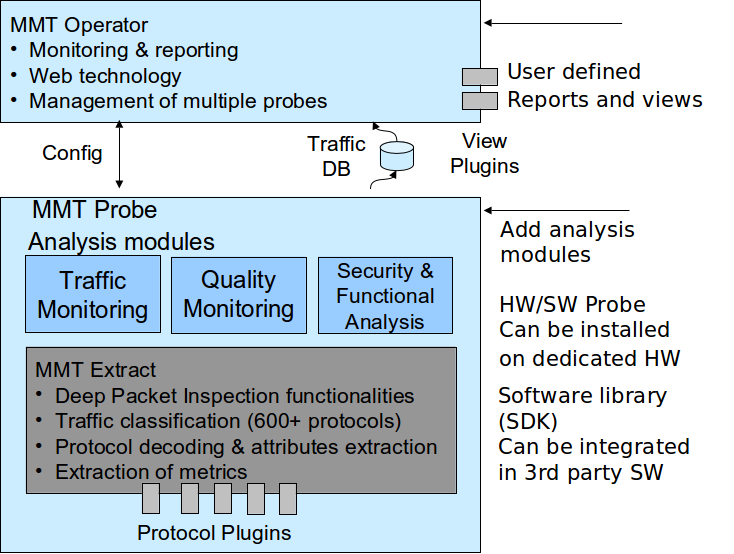
\includegraphics[width=3.8in]{img/archi.png}
\caption{MMT Architecture}\label{archi}
\end{figure}

The integrated {MMT} tool is composed of three complementary, but independent, modules as depicted in this figure.

\textbf{MMT-DPI} is the core packet\footnote{Note that the terms: {\textquotedblleft}packet{\textquotedblright}, {\textquotedblleft}message{\textquotedblright}, {\textquotedblleft}log entry{\textquotedblright} and {\textquotedblleft}event{\textquotedblright} can be considered as equivalent in this document. Here we will use either the term {\textquotedblleft}packet{\textquotedblright} or {\textquotedblleft}event{\textquotedblright} to denote an event in time that is perceived as structured data that can be extracted, classified and analysed.} processing module. It is a C library that analyses network traffic using Deep Packet/Flow Inspection (DPI/DFI) techniques in order to extract hundreds of network and application based events, including: protocols field values, data in messages and logs, network and application QoS parameters and KPIs. MMT-DPI incorporates a plugin architecture for the addition of new protocols and data structures; and, a public API for integrating third party probes (more details given in Section~\ref{Developers}).

\textbf{MMT-Security} is a security analysis engine based on MMT-Security properties described in this document. MMT-Security analyses and correlates network and application events to detect operational and security incidents. For each occurrence of a security property, MMT-Security allows to detect whether it was respected or violated.
The MMT-Security engine has been fully implemented in the context of Montimage{\textquoteright}s research projects. It is the result of previous research work in the network monitoring field and relies on the multi-domain security requirements identified in the context of diverse case studies (more details given in section~\ref{Other}). 

\textbf{MMT-Probe} is a main application that uses MMT-DPI and MMT-Security. It captures packets, makes them available to MMT-DPI and MMT-Security, and receives resulting values (extracted meta data or statistics) to be used for creating reports forwarded to MMT-Operator.

\textbf{MMT-Operator} is a visualization Web application. It allows collecting and aggregating meta data and reports provided by MMT-Probe, and presents them via a graphical user interface (e.g., alarms, line charts). MMT-Operator is customisable: the user is able to define new views or customise the large list of predefined ones. With its generic connector, MMT-Operator can also be integrated with third party traffic probes.



%****************************************************

%****************************************************
\subsection{Features}

\index{architecture}\marginlabel{Main features:} The main features provided by {MMT} are:
\begin{enumerate}
\item
\textit{Granular traffic analysis capabilities}: MMT allows parsing a wide range of protocols and applications and to extract various network and application based traffic performance indicators. The extraction is powered by a plugin architecture for the addition of new protocols and applications.

\item
\textit{Application classification}: Prior to extracting protocol or application attributes, MMT uses DPI techniques for application identification and classification. This is essential when analysing applications that use non-standard port numbers (e.g., P2P, Skype). 

\item
\textit{Rule engine}: MMT-Security introduces a rule engine that allows the detection of complex sequence of events that conventional monitoring does not detect. This is used to monitor: i) access control policies (e.g., that authorized users are authenticated prior to using a critical business application); ii) anomaly or attacks (e.g., excessive login attempts on the application server); iii) performance (e.g., identification of VoIP calls with QoS parameters exceeding acceptable quality thresholds); and, much more.

\item
\textit{Configurable reports}: MMT traffic reports and charts can be configured by the user. The user can edit pre-configured reports and create new ones. Different chart types and graphs can be used including: pie, histograms, time charts, stacked area charts, sequence charts, tables, hierarchical tables, etc.

\item
\textit{Multi-platform solution}: MMT is available and tested on Linux based distributions but portable on Windows. It can be installed as software on commodity hardware or optimized for integration with dedicated probes.

\item
\textit{Modular solution}: MMT is a modular solution composed of four components: MMT-DPI library for the traffic processing and data decoding; MMT-Security engine for property analysis; MMT-Probe application for integrating MMT-DPI and MMT-Security; and MMT-Operator for data aggregation, correlation, reporting, and distributed probe management. It is possible to integrate MMT-DPI and MMT-Security in third party traffic probes and to connect MMT-Operator with existing monitoring systems.
\end{enumerate}
%****************************************************


%%%%%%%%%%%%%%%%%%%%%%%%%%%%%%%%%%%%%%%%%%%%%%%%%%%%%%%%%%%%%%%%%%%%%%
